%%%%%%%%%%%%%%%%%%%%%%%%%%%%%%%%%%%%%%%%%%%%%%%%%%%%%%%%%%%%%%%%%%%%%
%%                                                                 %%
%% Please do not use \input{...} to include other tex files.       %%
%% Submit your LaTeX manuscript as one .tex document.              %%
%%                                                                 %%
%% All additional figures and files should be attached             %%
%% separately and not embedded in the \TeX\ document itself.       %%
%%                                                                 %%
%%%%%%%%%%%%%%%%%%%%%%%%%%%%%%%%%%%%%%%%%%%%%%%%%%%%%%%%%%%%%%%%%%%%%

%%\documentclass[referee,sn-basic]{sn-jnl}% referee option is meant for double line spacing

%%=======================================================%%
%% to print line numbers in the margin use lineno option %%
%%=======================================================%%

%%\documentclass[lineno,sn-basic]{sn-jnl}% Basic Springer Nature Reference Style/Chemistry Reference Style

%%======================================================%%
%% to compile with pdflatex/xelatex use pdflatex option %%
%%======================================================%%

%%\documentclass[pdflatex,sn-basic]{sn-jnl}% Basic Springer Nature Reference Style/Chemistry Reference Style

%%\documentclass[sn-basic]{sn-jnl}% Basic Springer Nature Reference Style/Chemistry Reference Style
\documentclass[sn-mathphys]{sn-jnl}% Math and Physical Sciences Reference Style
%%\documentclass[sn-aps]{sn-jnl}% American Physical Society (APS) Reference Style
%%\documentclass[sn-vancouver]{sn-jnl}% Vancouver Reference Style
%%\documentclass[sn-apa]{sn-jnl}% APA Reference Style
%%\documentclass[sn-chicago]{sn-jnl}% Chicago-based Humanities Reference Style
%%\documentclass[sn-standardnature]{sn-jnl}% Standard Nature Portfolio Reference Style
%%\documentclass[default]{sn-jnl}% Default
%%\documentclass[default,iicol]{sn-jnl}% Default with double column layout

%%%% Standard Packages
%%<additional latex packages if required can be included here>
%%%%

%%%%%=============================================================================%%%%
%%%%  Remarks: This template is provided to aid authors with the preparation
%%%%  of original research articles intended for submission to journals published 
%%%%  by Springer Nature. The guidance has been prepared in partnership with 
%%%%  production teams to conform to Springer Nature technical requirements. 
%%%%  Editorial and presentation requirements differ among journal portfolios and 
%%%%  research disciplines. You may find sections in this template are irrelevant 
%%%%  to your work and are empowered to omit any such section if allowed by the 
%%%%  journal you intend to submit to. The submission guidelines and policies 
%%%%  of the journal take precedence. A detailed User Manual is available in the 
%%%%  template package for technical guidance.
%%%%%=============================================================================%%%%

\jyear{2021}%

%% as per the requirement new theorem styles can be included as shown below
\theoremstyle{thmstyleone}%
\newtheorem{theorem}{Theorem}%  meant for continuous numbers
%%\newtheorem{theorem}{Theorem}[section]% meant for sectionwise numbers
%% optional argument [theorem] produces theorem numbering sequence instead of independent numbers for Proposition
\newtheorem{proposition}[theorem]{Proposition}% 
%%\newtheorem{proposition}{Proposition}% to get separate numbers for theorem and proposition etc.

\theoremstyle{thmstyletwo}%
\newtheorem{example}{Example}%
\newtheorem{remark}{Remark}%

\theoremstyle{thmstylethree}%
\newtheorem{definition}{Definition}%
\usepackage{ragged2e}
\raggedbottom
%%\unnumbered% uncomment this for unnumbered level heads

\begin{document}

\title[\textit{Detecting Fraud Calls vis-à-vis Natural Language Processing}]{Detecting Fraud Calls vis-à-vis Natural Language Processing}

%%=============================================================%%
%% Prefix	-> \pfx{Dr}
%% GivenName	-> \fnm{Joergen W.}
%% Particle	-> \spfx{van der} -> surname prefix
%% FamilyName	-> \sur{Ploeg}
%% Suffix	-> \sfx{IV}
%% NatureName	-> \tanm{Poet Laureate} -> Title after name
%% Degrees	-> \dgr{MSc, PhD}
%% \author*[1,2]{\pfx{Dr} \fnm{Joergen W.} \spfx{van der} \sur{Ploeg} \sfx{IV} \tanm{Poet Laureate} 
%%                 \dgr{MSc, PhD}}\email{iauthor@gmail.com}
%%=============================================================%%

\author*[1]{\fnm{Anurag} \sur{Dutta}}\email{anuragdutta.research@gmail.com}

% \equalcont{These authors contributed equally to this work.}

% \author[1,2]{\fnm{Third} \sur{Author}}
% \email{iiiauthor@gmail.com}
% \equalcont{These authors contributed equally to this work.}

\affil*[1]{Undergraduate, \orgdiv{Computer Science and Engineering}, \orgname{Government College of Engineering and Textile Technology}, \orgaddress{\street{12, William Carey Road}, \city{Serampore}, \postcode{712201}, \state{Calcutta}, \country{India}}}

%%==================================%%
%% sample for unstructured abstract %%
%%==================================%%

%\abstract{Fraud is defined in law as the willful use of deception to obtain unfair or illegal gain or to deny a victim of a legitimate right. Fraud can be illegal under criminal law or civil law. Scam may not always result in a loss of money, property, or legal rights but still be a component of another civil or criminal wrong. A victim of fraud may sue the offender to stop the fraud or receive monetary compensation. The goal of fraud may be financial gain or other benefits, such as getting a passport, travel document, or driver's licence, or it may be mortgage fraud, when the offender makes false claims in an effort to qualify for a mortgage. The collection of enormous volumes of data combined with predictive analytics or forensic analytics, the use of electronic data to reconstruct or detect fraud, makes the detection of fraudulent acts on a wide scale conceivable. Particularly when using computer-based analytical techniques, errors, inconsistencies, inefficiencies, irregularities, and biases can be exposed, which frequently pertain to fraudsters favouring particular currency amounts in order to bypass internal control thresholds. Scam calls are false calls that persons or businesses make in an effort to deceive recipients into parting with their money or private information. Scammers frequently play down the situation by calling it a normal call or even by lying to the person they were trying to con. In this work, we will try to detect fraud calls, by making use of Supervised Machine Learning Algorithms. For the same, we have collected a total of 5925 Data points. We have used the data to train the model. For obvious reasons, we have kept the source of the data as anonymous. This work would help in early detection of scam calls and would help a lot of innocent lives from getting tied by the knot of fraudulences. Numerous ML Algorithms have been used for the work, namely Support Vector Machine, $k$ - Nearest Neighbours, Gaussian Naive Bayes, etc. Further, these Algorithms have been compared on the basis of their performance of prediction. }

%%================================%%
%% Sample for structured abstract %%
%%================================%%

\abstract{\textbf{Purpose:} Fraud is defined in law as the willful use of deception to obtain unfair or illegal gain or to deny a victim of a legitimate right. Fraud can be illegal under criminal law or civil law. Scam may not always result in a loss of money, property, or legal rights but still be a component of another civil or criminal wrong. A victim of fraud may sue the offender to stop the fraud or receive monetary compensation. The goal of fraud may be financial gain or other benefits, such as getting a passport, travel document, or driver's licence, or it may be mortgage fraud, when the offender makes false claims in an effort to qualify for a mortgage. The collection of enormous volumes of data combined with predictive analytics or forensic analytics, the use of electronic data to reconstruct or detect fraud, makes the detection of fraudulent acts on a wide scale conceivable. Particularly when using computer-based analytical techniques, errors, inconsistencies, inefficiencies, irregularities, and biases can be exposed, which frequently pertain to fraudsters favouring particular currency amounts in order to bypass internal control thresholds. Scam calls are false calls that persons or businesses make in an effort to deceive recipients into parting with their money or private information. Scammers frequently play down the situation by calling it a normal call or even by lying to the person they were trying to con. In this work, we will try to detect fraud calls, by making use of Supervised Machine Learning Algorithms. For the same, we have collected a total of 5925 Data points. We have used the data to train the model. For obvious reasons, we have kept the source of the data as anonymous. This work would help in early detection of scam calls and would help a lot of innocent lives from getting tied by the knot of fraudulences. \\\textbf{\\}
% 
\textbf{Methods:} Numerous Machine Learning Algorithms have been used for the work, namely Support Vector Machine, $k$ - Nearest Neighbours, Gaussian Naive Bayes, etc. Further, these Algorithms have been compared on the basis of their performance of prediction. We have also used the corpus, from Natural Language Toolkit Python Library, for preprocessing of data. \\\textbf{\\}
% 
\textbf{Results:} According to the work proposed in the article, Support Vector Machine is best for detection of Fraud Calls, as the model modelled using Support Vector Classifier gives an accuracy of 97.9\%. \\\textbf{\\}
% 
\textbf{Conclusion:} Fraudulences have caught great height in current work of advancing informatics. The betterments in the Information Technology can be taken into account to avoid innocent people from getting trapped. Government can impose laws and regulations advising the Telecom Exchange companies to introduce the Scam Call Classifier Technique as their key element. This would adversely impact the surging rate of Fraudulence. 
}

\keywords{Supervised Learning, Support Vector Machine, Gaussian Naive Bayes, \textit{k} - Nearest Neighbours, Fraud Detection, Criminology, Natural Language Processing}

\pacs[JEL Classification]{C810, C820, O390}

%%\pacs[MSC Classification]{35A01, 65L10, 65L12, 65L20, 65L70}

\maketitle          % typeset the header of the contribution
%
\section{Introduction}
Fraud is a purposeful act of deception that leads to unethical or unfair behaviour, according to the law. Fraud is frequently categorised as a criminal offence. Fraudulent behaviour is motivated for a variety of causes. Others fabricate the assertions for their own personal gain, which cannot be done without committing a crime, while some people want to benefit from value.  According to the most popular definition, fraud is "a deception with the goal to benefit financially or personally." Different legal systems have different definitions of what constitutes a valid explanation for fraud, which may be a civil wrong requiring proof and a rationale, or a criminal infraction if the intentional deception has been justified. Financial scams are common and cost the people who commit them a lot of money. For instance, a business or bank may trick a customer into paying for extra services. The Wells Fargo bank in the United States experienced one of the same situations. A bank is the target of a bank fraud, which is typically carried out by making false claims and utilising fictitious documentation. Everyone is concerned about bank fraud. It is a highly delicate subject since it impacts public trust, which is the foundation of the entire banking system. The term "bank fraud" refers to a variety of thefts, embezzlements, and falsifications of negotiable documents such checks, bank draughts, bills of exchange, statements of accounts, stocks, etc. The booming banking industry has led to an increase in bank fraud. Indian Penal Code addresses bank fraud. By using a fake signature on the check, frauds are frequently conducted in the domain of checks. The majority of bank frauds presumably occur in this manner. Hypothecation fraud is another type of fraud in which money is fraudulently obtained in exchange for a security of some sort. A fair financial system that enjoys the public's confidence is a prerequisite for an equitable economic system. To prevent it, a number of preventive steps can be done, such as proper recruiting, constant attention, adherence to regulations, training programmes, etc. Telephonic Frauds are an another strata of Fraudulences that affect many people round the world. People are constantly communicating. Sadly, they don't always communicate in the most polite manner. While some attempts at communication result in violent or unpleasant interactions, other attempts at communication result in frauds. Scams occur on a variety of platforms, including the internet and the phone. An individual is frequently deceived into divulging personal information unknowingly when a fraud occurs. Although there are many other ways available, intimidation tactics are frequently used. In particular, the general public is compelled to accept criminals when they employ tech assistance as a front, lest they leave their computers vulnerable to malware attacks. In essence, there are many other types of scams, and this is just one of the most recent ones that customers should be aware of. Scams, whether they are conducted over the phone or in another way, need a vulnerability to operate. There are many different kinds of breaches, ranging from data to financial. The 2014 public awareness campaign on the Telephone Technical Support Scam involved an unintentional disclosure. Technical support frightened people into providing personal information when they contacted, leading them to believe they were chatting with experts who would clean their machines of malware or viruses. They also kept sending money to a person they thought was a government official after learning that the technical support was a hoax. Despite the fact that they shared information, they had no intention of sharing it with a fraudster. Studies make sure that the Telephonic Phone is compromising the security and privacy of many individuals. In this work, we would build a model that can predict a call as being Fraud or Normal. From the problem statement, it's clear that it's a classification problem. So, for modelling the same, we would make use of Supervised Learning Algorithms, like Gaussian Naive Bayes, Support Vector Machine, \textit{k} - Nearest Neighbours, etc. For solving any Machine Learning Problem, before we design the Model, we will have to pre-process the data. Since, the data may have a lot of noise, and nuisances, Natural Language Processing Techniques have been employed in our work to prepare the model that could lead to higher accuracies. 
\section{Dataset}
The Dataset, that we have used for the work, is a collection of 05925 Data points. To avoid compensation of private sources, the source of Dataset is kept private. Given are, a few instances of the dataset. Figure \ref{Fig. 1} explains the prediction mechanism of data points by the Machine Learning Algorithms. \\
\begin{verbatim}
----------------------------------------------------------------
INDEX  LABEL   FEATURE
----------------------------------------------------------------
0      fraud   Hello, i m bank manager of SBI, ur debit card ...
1      fraud   Todays Vodafone numbers ending with 4882 are s...
2      normal  Please don't say like that. Hi hi hi
3      normal  Thank you!
4      normal  Oh that was a forwarded message. I thought you...
..      ..       ..
..      ..       ..
..      ..       ..
5920   fraud   to get 1000 INR voucher please call on 8898655...
5921   fraud   to get free access of google cloud account hit...
5922   fraud   to get free AWS cloud account hit on given mes...
5923   fraud   to get free access of Microsoft Azure hit on g...
5924   fraud   hello sir, we are from your bank have you fill...
----------------------------------------------------------------
\end{verbatim}
\textbf{\\}Machine Learning Algorithms takes feature as input, and returns back the Label as an output. 
\begin{figure}[!h]
\centering
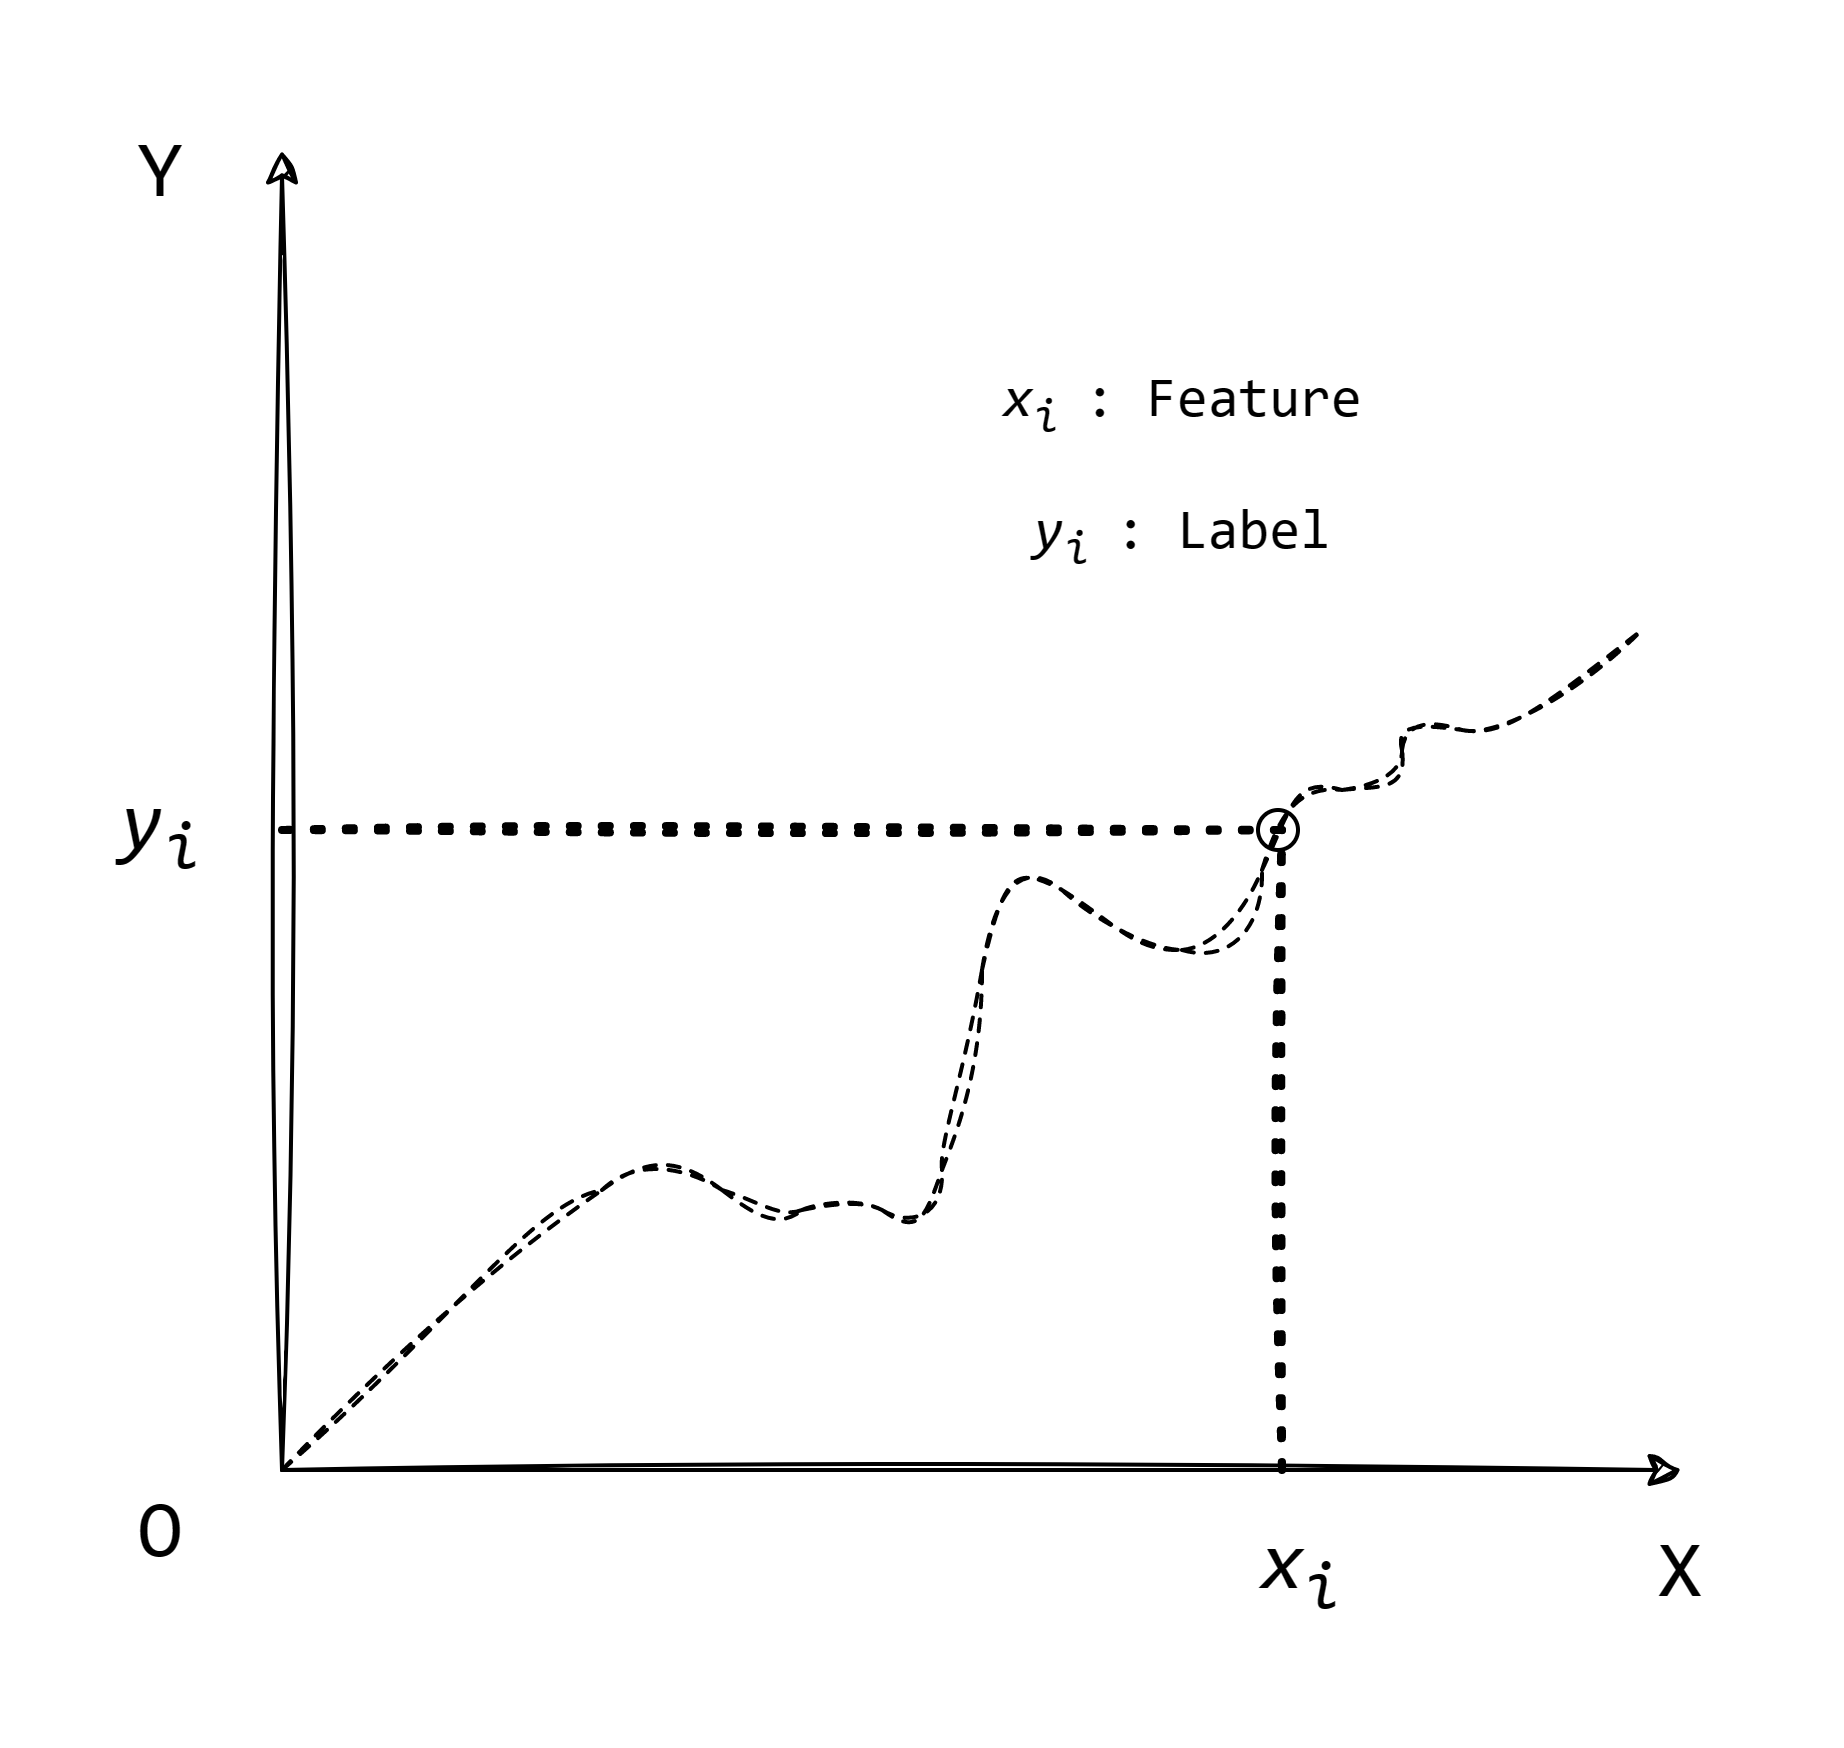
\includegraphics[width=\textwidth]{1}
\label{fig1}
\caption{Machine Learning Algorithms to Predict Label from a Feature. Algorithms, take the feature, $x_i$ as input, and predict the label, $y_i$ as output. The performance of the Machine Learning Algorithms is a measure of how well does the curve mimic the real time scenario. The equation representing the curve is $y = \phi(x) + \epsilon$. $\phi(x)$ is also known as Target Function, and $\epsilon$ is the Error Term.}
\label{Fig. 1}
\end{figure}
\section{Natural Language Processing}
The study of how computers interact with human language, particularly how to design computers to process and analyse huge amounts of natural language data, is known as natural language processing (NLP), an interdisciplinary subject of linguistics, computer science, and artificial intelligence. The ultimate goal is to create a machine that is able to "understand" the contents of documents, including the subtle subtleties of language used in different contexts. Once the information and insights are accurately extracted from the documents, the technology can classify and arrange the documents themselves. In many different commercial disciplines and places, personal assistants employ this technology. The system analyses the verbal input from the user, deconstructs it for accurate comprehension, and then processes it as necessary. Due to the fact that it is a very current and successful strategy, there is a huge demand for it right now. It has already been possible to have interactive conversations with a human being and work with smart devices thanks to advancements in the field of natural language processing. The focus of AI applications in NLP was on knowledge representation, logical reasoning, and constraint fulfilment. Here, it was used first for semantics and then for grammar. A dramatic shift in NLP research over the past ten years has led to the extensive use of statistical techniques like machine learning and data mining. Due to the amount of work that needs to be done these days, automation is constantly needed. When it comes to automated applications, NLP is a really positive component. NLP is one of the most popular ways to deploy machine learning due of its applications. In order to better understand how computers and people communicate using natural language, the area of "natural language processing" (NLP) combines computer science, linguistics, and machine learning. The objective of NLP is to enable computers to comprehend and produce human language. This not only increases the effectiveness of human work but also facilitates communication with machines. NLP fills the communication gap between people and machines. The Natural Language Toolkit, or more simply NLTK, is a collection of Python-coded tools and applications for symbolic and statistical natural language processing (NLP) of English. It was created by Steven Bird and Edward Loper at the University of Pennsylvania's Department of Computer and Information Science. NLTK contains sample data and graphical demos. In addition to a cookbook, it comes with a book that describes the fundamental ideas behind the language processing jobs that the toolkit supports. The goal of NLTK is to facilitate research and instruction in NLP or closely related fields including information retrieval, cognitive science, artificial intelligence, and empirical linguistics. NLTK has been effectively used as a teaching tool, a tool for solitary study, and as a foundation for developing research systems. 25 nations, including 32 colleges in the US, use NLTK in their classes. Functionalities for categorising, tokenizing, stemming, tagging, parsing, and semantic reasoning are supported by NLTK. According to it's Stable Release available at GitHub, NLTK source code is distributed under the $\mathtt{Apache}$  $\mathtt{2.0}$ $\mathtt{License}$.and the documentation is distributed under the $\mathtt{Creative}$ $\mathtt{Commons}$ $\mathtt{3.0}$ license.
\end{document}
